\documentclass{article}
\usepackage{amsfonts, amsthm, amsmath, amssymb, mathtools, ulem, mathrsfs, physics, esint, siunitx, tikz-cd}
\usepackage{pdfpages, fullpage, color, microtype, cancel, textcomp, markdown, hyperref, graphicx}
\usepackage{enumitem}
\usepackage{algorithm}
\usepackage{algpseudocode}
\graphicspath{{./images/}}
\usepackage[english]{babel}
\usepackage[autostyle, english=american]{csquotes}
\MakeOuterQuote{"}
\usepackage{xparse}
\usepackage{tikz}

\usepackage{calligra}
\DeclareMathAlphabet{\mathcalligra}{T1}{calligra}{m}{n}
\DeclareFontShape{T1}{calligra}{m}{n}{<->s*[2.2]callig15}{}
\newcommand{\script}[1]{\ensuremath{\mathcalligra{#1}}}
\newcommand{\scr}{\script r}

% fonts
\def\mbb#1{\mathbb{#1}}
\def\mfk#1{\mathfrak{#1}}
\def\mbf#1{\mathbf{#1}}
\def\tbf#1{\textbf{#1}}

% common bold letters
\def\bP{\mbb{P}}
\def\bC{\mbb{C}}
\def\bH{\mbb{H}}
\def\bI{\mbb{I}}
\def\bR{\mbb{R}}
\def\bQ{\mbb{Q}}
\def\bZ{\mbb{Z}}
\def\bN{\mbb{N}}

% brackets
\newcommand{\br}[1]{\left(#1\right)}
\newcommand{\sbr}[1]{\left[#1\right]}
\newcommand{\brc}[1]{\left\{#1\right\}}
\newcommand{\lbr}[1]{\left\langle#1\right\rangle}

% vectors
\renewcommand{\i}{\hat{\imath}}
\renewcommand{\j}{\hat{\jmath}}
\renewcommand{\k}{\hat{k}}
\newcommand{\proj}[2]{\text{proj}_{#2}\br{#1}}
\newcommand{\m}[2][b]{\begin{#1matrix}#2\end{#1matrix}}
\newcommand{\arr}[3][\sbr]{#1{\begin{array}{#2}#3\end{array}}}

% misc
\NewDocumentCommand{\seq}{O{n} O{1} O{\infty} m}{\br{#4}_{{#1}={#2}}^{#3}}
\NewDocumentCommand{\app}{O{x} O{\infty}}{\xrightarrow{#1\to#2}}
\newcommand{\sm}{\setminus}
\newcommand{\sse}{\subseteq}
\renewcommand{\ss}{\subset}
\newcommand{\vn}{\varnothing}
\newcommand{\lc}{\epsilon_{ijk}}
\newcommand{\ep}{\epsilon}
\newcommand{\vp}{\varphi}
\renewcommand{\th}{\theta}
\newcommand{\cjg}[1]{\overline{#1}}
\newcommand{\inv}{^{-1}}
\DeclareMathOperator{\im}{im}
\DeclareMathOperator{\id}{id}
\newcommand{\ans}{\tbf{Ans. }}
\newcommand{\pf}{\tbf{Pf. }}
\newcommand{\imp}{\implies}
\newcommand{\impleft}{\reflectbox{$\implies$}}
\newcommand{\ck}{\frac1{4\pi\ep_0}}
\newcommand{\ckb}{4\pi\ep_0}
\newcommand{\sto}{\longrightarrow}
\DeclareMathOperator{\cl}{cl}
\DeclareMathOperator{\intt}{int}
\DeclareMathOperator{\bd}{bd}
\DeclareMathOperator{\Span}{span}
\newcommand{\floor}[1]{\left\lfloor#1\right\rfloor}
\newcommand{\ceil}[1]{\left\lceil#1\right\rceil}
\newcommand{\fxn}[5]{#1:\begin{array}{rcl}#2&\longrightarrow & #3\\[-0.5mm]#4&\longmapsto &#5\end{array}}
\newcommand{\sep}[1][.5cm]{\vspace{#1}}
\DeclareMathOperator{\card}{card}
\renewcommand{\ip}[2]{\lbr{#1,#2}}
\renewcommand{\bar}{\overline}
\DeclareMathOperator{\cis}{cis}
\DeclareMathOperator{\Arg}{Arg}
\newcommand{\om}{\omega}
\DeclareMathOperator{\diag}{diag}

% title
\title{Scientific Computing HW 4}
\author{Ryan Chen}
%\date{\today}
\setlength{\parindent}{0pt}


\begin{document}
	
\maketitle



\tbf{Problem 1.} \pf The characteristic polynomial is
$$\rho(z) = z^k + \sum_{j=0}^{k-1}\alpha_jz^{k-1-j}$$
and the recurrence is
$$u_{n+1} + \sum_{j=0}^{k-1}\alpha_ju_{n-j} = 0$$
Define a linear operator $D:=r\dv{r}$. Then for all $n$ and $l$,
$$D[n^lr^n] = r\dv{r} n^lr^n = rn^lnr^{n-1} = n^{l+1}r^n$$
so that in particular,
$$n^lr^n = D[n^{l-1}r^n] = D^2[n^{l-2}r^n] = \ldots = D^l[r^n] \quad (1.1)$$
Plug $u_n=n^lr^n$ into the LHS of the recurrence, apply (1.1) to each term, then use the linearity of $D$.
$$u_{n+1} + \sum_{j=0}^{k-1}\alpha_ju_{n-j} = (n+1)^lr^{n+1} + \sum_{j=0}^{k-1}\alpha_j(n-j)^lr^{n-j}
= D^l[r^{n+1}] + \sum_{j=0}^{k-1}\alpha_j D^l[r^{n-j}]
= D^l\sbr{r^{n+1} + \sum_{j=0}^{k-1}\alpha_j r^{n-j}}$$
$$= D^l\sbr{r^{n-k+1}\br{r^k + \sum_{j=0}^{k-1}\alpha_jr^{k-1-j}}}
= D^l[r^{n-k+1}\rho(r)]
= D^l[0]
= 0$$
\sep



\tbf{Problem 2.} \pf We first establish a lemma. For the $(k-1)\times k$ matrix
$$\m{\lambda & -1 \\ & \lambda & -1 \\ & & \ddots & \ddots \\ & & & \lambda & -1}$$
The submatrix formed by deleting the $j$th column has determinant $(-1)^{k-j}\lambda^{j-1}$. To see this, write the submatrix in block form.
$$M :=
	\m{\m[]{\lambda & -1 \\ & \lambda & -1 \\ & & \ddots & \ddots \\ & & & \lambda & -1 \\ & & & & \lambda}
	& 0_{(j-1)\times(k-j)} \\
	0_{(k-j)\times(j-1)}
	& \m[]{-1 \\ \lambda & -1 \\ & \ddots & \ddots \\ & & \lambda & -1}}$$
Using the fact that
$$\det \m{B & 0 \\ 0 & C} = \det(B)\det(C)$$
we have $\det M = \lambda^{j-1}(-1)^{k-j}$.\\

We now aim to show $\det(\lambda I-A)=\rho(\lambda)$.
$$\lambda I-A = \m{
\lambda & -1\\
& \lambda & -1\\
& & \ddots & \ddots\\
& & & \lambda & -1\\
\alpha_{k-1} & \alpha_{k-2} & \dots & \alpha_1 & \lambda+\alpha_0
}$$
Expanding over row $k$, starting at column $k$, and using the above lemma,
$$\det(\lambda I-A)
= (\lambda+\alpha_0)(-1)^{k-k}\lambda^{k-1} + \sum_{j=1}^{k-1}(-1)^{k+k-j}\alpha_j(-1)^{k-k+j}\lambda^{k-j-1}
= \lambda^k + \alpha_0\lambda^{k-1} + \sum_{j=1}^{k-1}(-1)^{2k}\alpha_j\lambda^{k-j-1}$$
$$= \lambda^k + \alpha_0\lambda^{k-1} + \sum_{j=1}^{k-1}\alpha_j\lambda^{k-j-1}
= \lambda^k + \sum_{j=0}^{k-1}\alpha_j\lambda^{k-j-1}
= \rho(\lambda)$$
\sep



\tbf{Problem 3.} Note: For explicit matrix norm computations we will use the Euclidean norm
$$\norm{A} = \sbr{\sum_{i,j}A_{ij}^2}^{1/2}$$

\pf Write the Jordan form of $A$.
$$A = SJS\inv,
\quad J = \diag(J_1,J_2,\dots,J_s),
\quad J_q = r_qI_{m_q} + N_q,
\quad N_q \overset{m_q\times m_q}{=} \m{
0 & 1 & & \\
& 0 & 1 & & \\
& & \ddots & \ddots \\
& & & 0 & 1
}$$
For all $p$,
$$A^p = SJ^pS\inv,
\quad J^p = \diag(J_1^p,J_2^p,\dots,J_s^p)$$
so we seek a bound on $\norm{J^p}$, where $J=rI+N$ is a Jordan block for an eigenvalue $r$ with multiplicity $m$ (we temporarily use $J$ to denote a single block instead of the whole matrix).\\

If $m=1$ then $J=[r]$, and since $\rho$ satisfies the root condition, $|r|\le 1$, giving
$$\norm{J^p} = |r|^p \le 1$$
Now say $m>1$, so that $|r|<1$ by the root condition. If $r=0$ then $J=N$, hence $\norm{J^p}=0$ for all $p\ge m$. Now say $r\ne 0$. For $p\ge m$,
$$J^p = (rI+N)^p = \sum_{j=0}^p \binom{p}{j}r^{p-j}N^j = \sum_{j=0}^m \binom{p}{j}r^{p-j}N^j$$
$$\imp \norm{J^p} \le \sum_{j=0}^p \binom{p}{j}|r|^{p-j}\norm{N^j}$$
Fix $j$ with $0\le j\le m$. We establish a bound on $\binom{p}{j}|r|^{p-j}$. Note
$$\binom{p}{j}|r|^{p-j} = \frac{p!}{j!(p-j)!}|r|^p|r|^{-j}
= \frac{1}{|r|^jj!}|r|^p \prod_{i=0}^{j-1}(p-i)
= \frac{1}{|r|^jj!} \cdot \frac{\prod_{i=0}^{j-1}(p-i)}{|1/r|^p}$$
Considering the fraction in the RHS as $p\to\infty$, the denominator, an exponential in $p$ with base $|1/r|>1$, grows faster than the numerator, a polynomial in $p$. This means $\binom{p}{j}|r|^{p-j}$ tends to 0 as $p\to\infty$, hence it has a bound $M_j$ independent of $p$.\\

Writing small powers of $N$,
$$N^0 = I = \m{
	1 &  & & \\
	& 1 &  & & \\
	& & \ddots &  \\
	& & & 1 & 
},
\quad N = \m{
	0 & 1 & & \\
	& 0 & 1 & & \\
	& & \ddots & \ddots \\
	& & & 0 & 1
},
\quad N^2 = \m{
	0 & 0 & 1 & \\
	& 0 & 0 & 1 & \\
	& & 0 & \ddots & 1 \\
	& & & 0 & 0
},
\quad N^3 = \m{
	0 & 0 & 0 & 1 \\
	& 0 & 0 & 0 & 1 \\
	& & 0 & 0 & 0 \\
	& & & 0 & 0
}
$$
we see that for $0\le j\le m$,
$$\norm{N^j} = \sbr{\sum_{i,j}(N^j)_{ij}^2}^{1/2} = [m-j]^{1/2} \le m^{1/2}$$

We have a bound on $\norm{J^p}$ independent of $p$. Here we re--introduce the subscript $q$.
$$\norm{J_q^p} \le \max\sbr{\norm{J_q^1},\norm{J_q^2},\dots,\norm{J_q^{m_q-1}},\sum_{j=0}^{m_q} M_{q,j} m_q^{1/2}} =: K_q$$
Now looking at the whole Jordan matrix $J$,
$$\norm{J^p} \le \sum_{q=1}^s \norm{J_q^p} \le \sum_{q=1}^s K_q$$
Thus
$$\norm{A^p} \le \norm{S}\norm{S\inv} \sum_{q=1}^s K_q$$
\sep



\tbf{Problem 4.} Plug the supposed solution $U_n$ into the LHS of the recurrence.
$$U_{n+1} = A^{n-k+2}U_{k-1} + h\sum_{j=0}^{n+1-k}A^jG_{n-j}
= A^{n-k+2}U_{k-1} + hG_n + h\sum_{j=1}^{n+1-k}A^jG_{n-j}$$
$$= A^{n-k+2}U_{k-1} + hG_n + h\sum_{j=0}^{n-k}A^{j+1}G_{n-j-1}$$
Plug the solution into the RHS.
$$AU_n + hG_n = A^{n-k+2}U_{k-1} + h\sum_{j=0}^{n-k}A^{j+1}G_{n-j-1} + hG_n$$
The two expressions are equal, so $U_n$ indeed solves the recurrence.
\sep



\tbf{Problem 5.}

\begin{enumerate}[label=(\alph*)]
	
\item \pf For BDF2, the interpolant is
$$p(t) = y_{n+1} + y[t_{n+1},t_n](t-t_{n+1}) + y[t_{n+1},t_n,t_{n-1}](t-t_{n+1})(t-t_n)$$
The derivative of the last term at $t_{n+1}$ is
$$\dv{t}\eval_{t=t_{n+1}} (t-t_{n+1})(t-t_n)
= (t-t_{n})+(t-t_{n+1})\eval_{t=t_{n+1}}
= 2t_{n+1}-t_{n}-t_{n+1}
= t_{n+1}-t_n
= h_n$$
and so
$$p'(t_{n+1}) = y[t_{n+1},t_n] + y[t_{n+1},t_n,t_{n-1}]h_n$$
Equating this with $f_{n+1}:=f(t_{n+1},u_{n+1})$ gives the BDF2 method.
$$\frac{u_{n+1}-u_n}{h_n} + \frac{\frac{u_{n+1}-u_n}{h_n} - \frac{u_n-u_{n-1}}{h_{n-1}}}{h_n+h_{n-1}}h_n = f_{n+1}$$
From $h_n=t_{n+1}-t_n$ and $\om=\frac{h_n}{h_{n-1}}$,
$$1 + \om = 1 + \frac{h_n}{h_{n-1}} = \frac{h_{n-1}+h_n}{h_{n-1}}
\imp (1+\om)^2 = \frac{1}{h_{n-1}^2}\sbr{h_{n-1}^2+h_n^2+2h_{n-1}h_n} \quad (5.1)$$
$$1 + 2\om = 1 + 2\frac{h_n}{h_{n-1}} = \frac{h_{n-1}+2h_n}{h_{n-1}} \quad (5.2)$$
From (5.1) and (5.2),
$$\frac{(1+\om)^2}{1+2\om} = \frac{h_{n-1}}{h_{n-1}+2h_n}\frac{1}{h_{n-1}^2}\sbr{h_{n-1}^2+h_n^2+2h_{n-1}h_n}
= \frac{1}{h_{n-1}+2h_n}\sbr{h_{n-1}+\frac{h_n^2}{h_{n-1}}+2h_n}$$
$$= h_{n-1}(1+2\om)\sbr{h_{n-1}+\frac{h_n^2}{h_{n-1}}+2h_n} \quad (5.3)$$
Now multiply the method by $h_n(h_n+h_{n-1})$.
$$(u_{n+1}-u_n)(h_n+h_{n-1}) + \sbr{\frac{u_{n+1}-u_n}{h_n} - \frac{u_n-u_{n-1}}{h_{n-1}}}h_n^2 = h_n(h_n+h_{n-1})f_{n+1}$$
Collect coefficients of the following terms. Rewrite them using (5.2) and (5.3).
\begin{align*}
	u_{n+1} &: \quad h_n + h_{n-1} + \frac{h_n^2}{h_n} = 2h_n + h_{n-1} \overset{(5.2)}{=} h_{n-1}(1+2\om) \\
	u_n &: \quad -(h_n + h_{n-1}) + \sbr{-\frac{1}{h_n} - \frac{1}{h_{n-1}}}h_n^2 = -\sbr{2h_n + h_{n-1} + \frac{h_n^2}{h_{n-1}}} \overset{(5.3)}{=} -h_{n-1}(1+2\om)\frac{(1+\om)^2}{1+2\om} \\
	u_{n-1} &: \quad \frac{h_n^2}{h_{n-1}} = h_{n-1}\om^2
\end{align*}
Putting these together, the method is
$$h_{n-1}(1+2\om)u_{n+1} - h_{n-1}(1+2\om)\frac{(1+\om)^2}{1+2\om}u_n + h_{n-1}\om^2 = h_n(h_n+h_{n-1})f_{n+1}$$
Divide by $h_{n-1}(1+2\om)$.
$$u_{n+1} - \frac{(1+\om)^2}{1+2\om}u_n + \frac{\om^2}{1+2\om}u_{n-1} = h_n\frac{\frac{h_n}{h_{n-1}}+1}{1+2\om}f_{n+1}
= h_n\frac{1+\om}{1+2\om}f_{n+1}$$


\item From the LHS of the method, define
$$\rho(z) := z^2 - \frac{(1+\om)^2}{1+2\om}z + \frac{\om^2}{1+2\om}$$
By Vieta's formulas, the roots $r,s$ of $\rho$ satisfy
$$r + s = \frac{(1+\om)^2}{1+2\om} = \frac{1+\om^2+2\om}{1+2\om} = \frac{\om^2}{1+2\om} + 1$$
$$rs = \frac{\om^2}{1+2\om}$$
From these we see
$$r = \frac{\om^2}{1+2\om},
\quad s = 1$$
Since $\om<1+\sqrt2$,
$$w^2 < (1+\sqrt2)^2 = 1 + 2 + 2\cdot\sqrt2 = 1 + 2(1+\sqrt2) = 1 + 2\om
\imp 0 \le r = \frac{\om^2}{1+2\om} < 1
\imp |r|<1$$
This leaves $s=1$ as the only root with modulus 1, and it has multiplicity 1. Thus $\rho$ satisfies the root condition, hence the method is stable.

\end{enumerate}
\sep



\tbf{Problem 6.} Code: \url{https://github.com/RokettoJanpu/Scientific-Computing-2/blob/main/hw4.ipynb}\\

A timestep of $h=10^{-3}$ was used. The CPU time for DIRK2 was about 2.673 seconds, while the CPU time for BDF2 was about 2.015 seconds. The time evolution of the individual components is shown below.

\begin{center}
	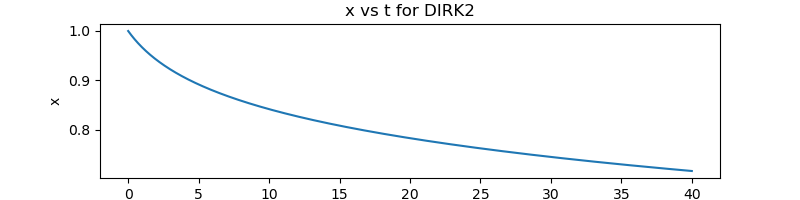
\includegraphics[scale=.25]{hw4 dirk x}
	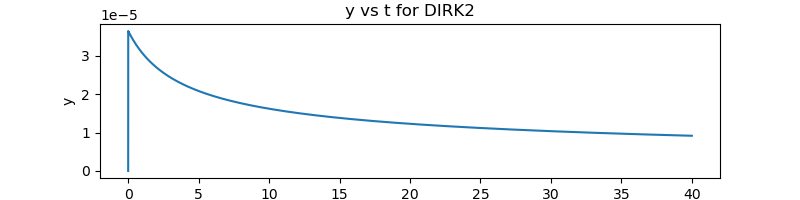
\includegraphics[scale=.25]{hw4 dirk y}
	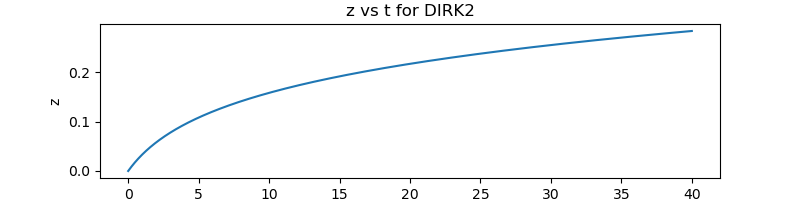
\includegraphics[scale=.25]{hw4 dirk z}
\end{center}
\begin{center}
	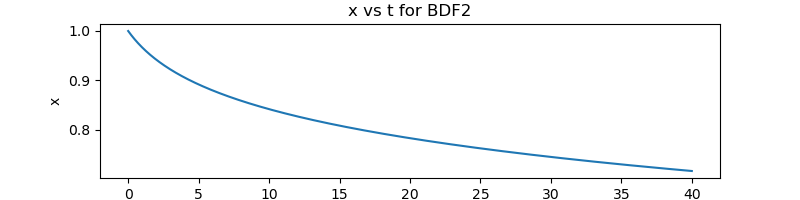
\includegraphics[scale=.25]{hw4 bdf x}
	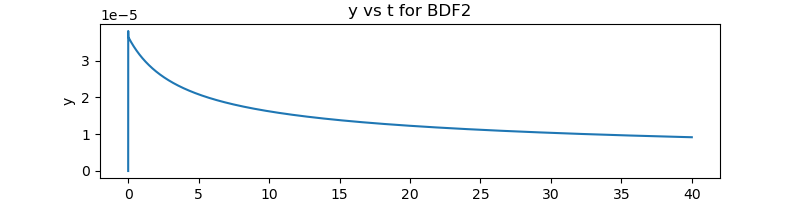
\includegraphics[scale=.25]{hw4 bdf y}
	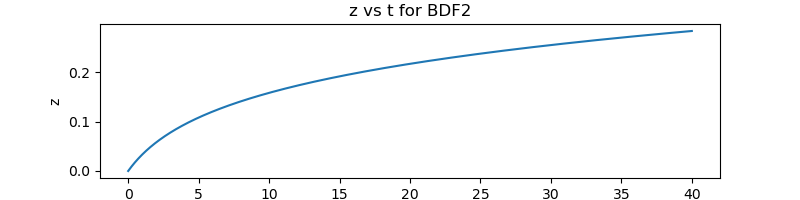
\includegraphics[scale=.25]{hw4 bdf z}
\end{center}

\end{document}